\documentclass[border=8mm]{standalone}
\usepackage[utf8]{inputenc}
\usepackage[T1]{fontenc}
\usepackage[scaled=0.92]{helvet}
\renewcommand{\familydefault}{\sfdefault}
\usepackage{xcolor}
\usepackage{tikz}
\usetikzlibrary{arrows.meta,shadows}
\definecolor{urjc}{RGB}{200,16,46}
\definecolor{marco}{RGB}{250,214,214}
\definecolor{curr}{RGB}{210,226,250}
\definecolor{acc}{RGB}{214,238,214}
\definecolor{eval}{RGB}{255,234,196}
\begin{document}
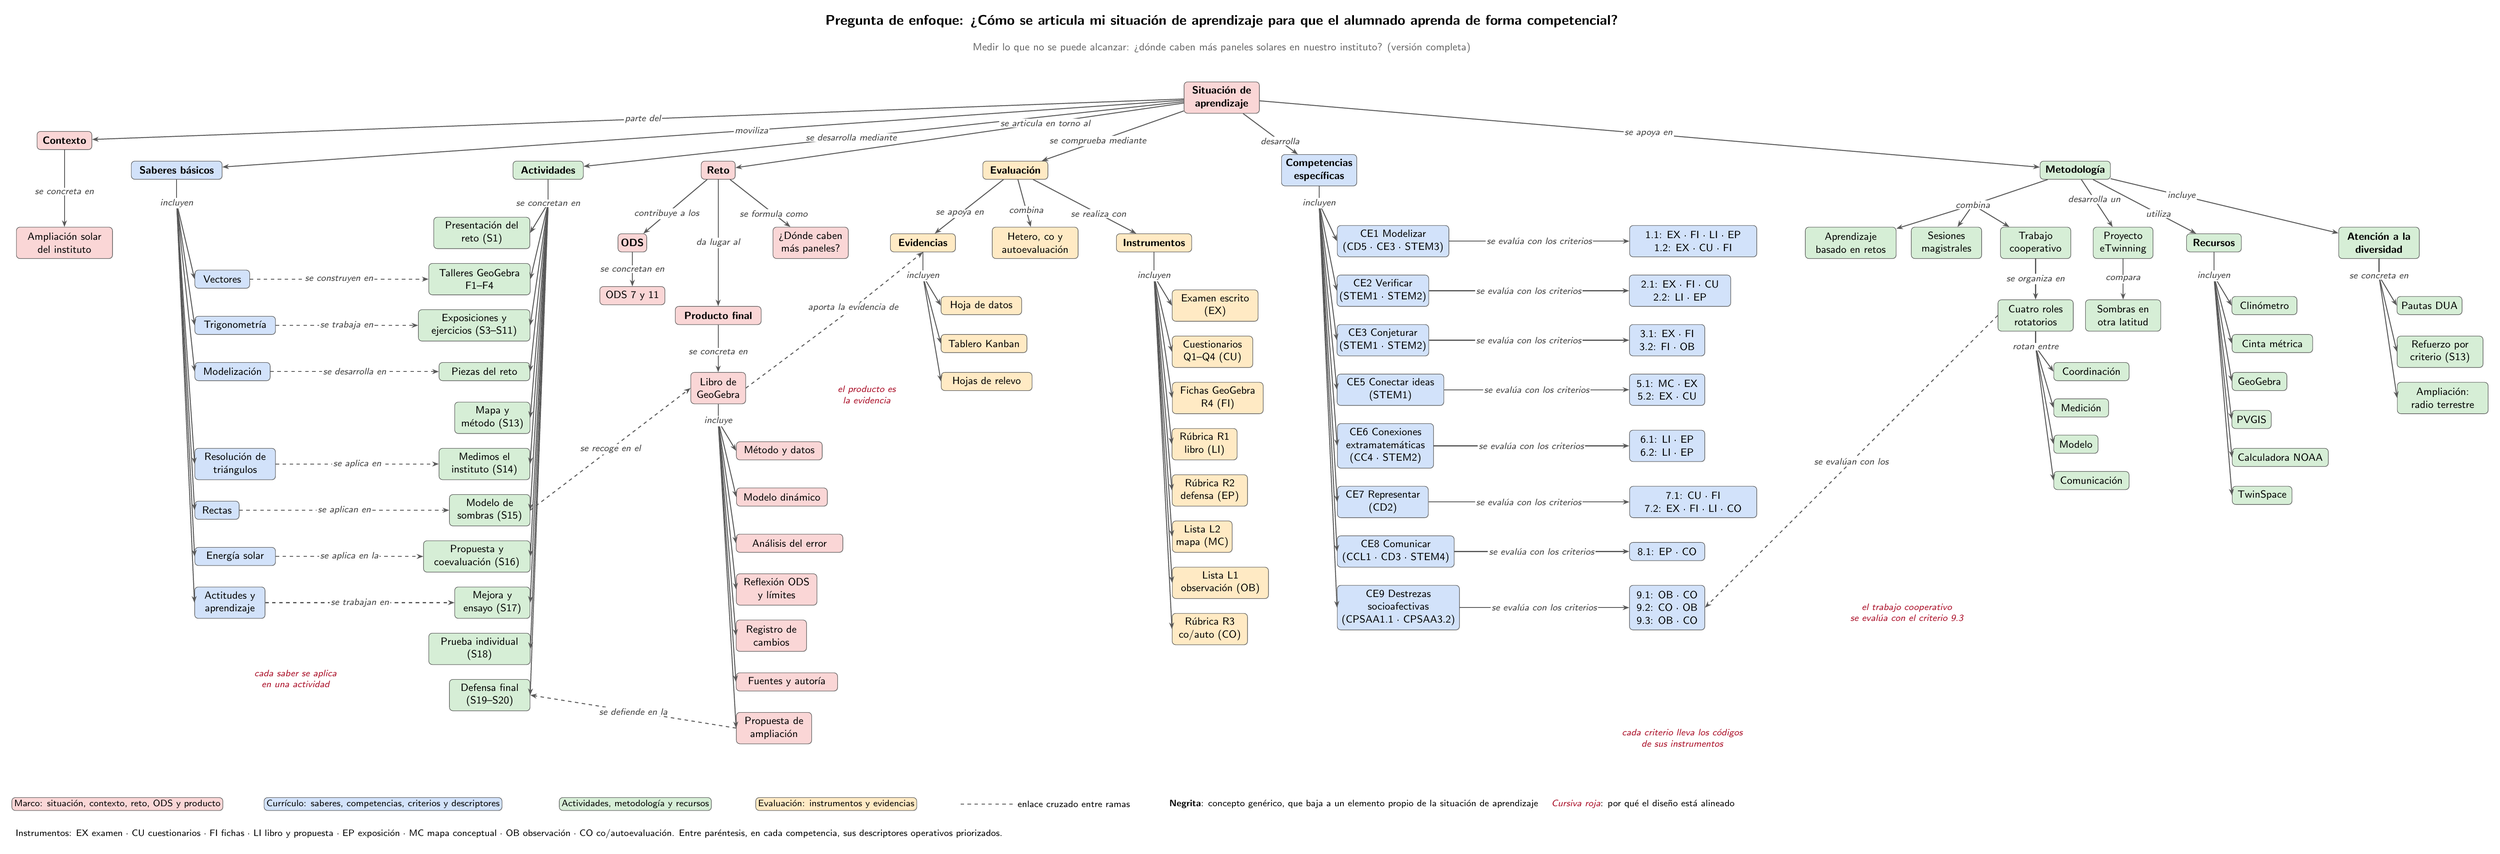
\begin{tikzpicture}[y=-1cm, font=\small,
  c/.style={draw=black!70, rounded corners=3pt, align=center, inner sep=2pt, fill=#1,
    drop shadow={opacity=0.15, shadow xshift=0.6pt, shadow yshift=-0.6pt}},
  lp/.style={fill=white, inner sep=1pt, font=\footnotesize\itshape, text=black!75},
  glosa/.style={font=\footnotesize\itshape, text=urjc!85!black, align=center},
  a/.style={-{Stealth[length=2mm]}, black!65, thick},
  l/.style={black!65, thick},
  cz/.style={dashed}]
\node[font=\large\bfseries] at (36.65,-2.3) {Pregunta de enfoque: ¿Cómo se articula mi situación de aprendizaje para que el alumnado aprenda de forma competencial?};
\node[text=black!60] at (36.65,-1.5) {Medir lo que no se puede alcanzar: ¿dónde caben más paneles solares en nuestro instituto? (versión completa)};
\node[c=marco, font=\small\bfseries, minimum width=2.28cm, minimum height=0.95cm] (sa) at (36.65,0.00) {Situación de\\aprendizaje};
\node[c=marco, font=\small\bfseries, minimum width=1.66cm, minimum height=0.55cm] (ctx) at (1.60,1.30) {Contexto};
\node[c=marco, font=\small, minimum width=2.91cm, minimum height=0.95cm] (ctx1) at (1.60,4.40) {Ampliación solar\\del instituto};
\node[c=curr, font=\small\bfseries, minimum width=2.75cm, minimum height=0.55cm] (sab) at (5.00,2.20) {Saberes básicos};
\node[c=curr, font=\small, minimum width=1.66cm, minimum height=0.55cm] (vec) at (6.38,5.50) {Vectores};
\node[c=curr, font=\small, minimum width=2.44cm, minimum height=0.55cm] (tri) at (6.77,6.90) {Trigonometría};
\node[c=curr, font=\small, minimum width=2.28cm, minimum height=0.55cm] (modz) at (6.69,8.30) {Modelización};
\node[c=curr, font=\small, minimum width=2.44cm, minimum height=0.95cm] (triang) at (6.77,11.10) {Resolución de\\triángulos};
\node[c=curr, font=\small, minimum width=1.34cm, minimum height=0.55cm] (rec) at (6.22,12.50) {Rectas};
\node[c=curr, font=\small, minimum width=2.44cm, minimum height=0.55cm] (energ) at (6.77,13.90) {Energía solar};
\node[c=curr, font=\small, minimum width=2.13cm, minimum height=0.95cm] (actit) at (6.61,15.30) {Actitudes y\\aprendizaje};
\node[c=acc, font=\small\bfseries, minimum width=2.13cm, minimum height=0.55cm] (act) at (16.25,2.20) {Actividades};
\node[c=acc, font=\small, minimum width=2.91cm, minimum height=0.95cm] (s1) at (14.24,4.10) {Presentación del\\reto (S1)};
\node[c=acc, font=\small, minimum width=3.07cm, minimum height=0.95cm] (f14) at (14.17,5.50) {Talleres GeoGebra\\F1–F4};
\node[c=acc, font=\small, minimum width=3.38cm, minimum height=0.95cm] (expo) at (14.01,6.90) {Exposiciones y\\ejercicios (S3–S11)};
\node[c=acc, font=\small, minimum width=2.75cm, minimum height=0.55cm] (piezas) at (14.32,8.30) {Piezas del reto};
\node[c=acc, font=\small, minimum width=2.28cm, minimum height=0.95cm] (s13) at (14.56,9.70) {Mapa y\\método (S13)};
\node[c=acc, font=\small, minimum width=2.75cm, minimum height=0.95cm] (med) at (14.32,11.10) {Medimos el\\instituto (S14)};
\node[c=acc, font=\small, minimum width=2.44cm, minimum height=0.95cm] (mod) at (14.48,12.50) {Modelo de\\sombras (S15)};
\node[c=acc, font=\small, minimum width=3.23cm, minimum height=0.95cm] (s16) at (14.09,13.90) {Propuesta y\\coevaluación (S16)};
\node[c=acc, font=\small, minimum width=2.28cm, minimum height=0.95cm] (s17) at (14.56,15.30) {Mejora y\\ensayo (S17)};
\node[c=acc, font=\small, minimum width=3.07cm, minimum height=0.95cm] (s18) at (14.17,16.70) {Prueba individual\\(S18)};
\node[c=acc, font=\small, minimum width=2.44cm, minimum height=0.95cm] (s19) at (14.48,18.10) {Defensa final\\(S19–S20)};
\node[c=marco, font=\small\bfseries, minimum width=1.03cm, minimum height=0.55cm] (reto) at (21.40,2.20) {Reto};
\node[c=marco, font=\small, minimum width=2.28cm, minimum height=0.95cm] (preg) at (24.20,4.40) {¿Dónde caben\\más paneles?};
\node[c=marco, font=\small\bfseries, minimum width=0.87cm, minimum height=0.55cm] (ods) at (18.80,4.40) {ODS};
\node[c=marco, font=\small, minimum width=1.97cm, minimum height=0.55cm] (ods711) at (18.80,6.00) {ODS 7 y 11};
\node[c=marco, font=\small\bfseries, minimum width=2.60cm, minimum height=0.55cm] (prod) at (21.40,6.60) {Producto final};
\node[c=marco, font=\small, minimum width=1.66cm, minimum height=0.95cm] (libro) at (21.40,8.80) {Libro de\\GeoGebra};
\node[c=marco, font=\small, minimum width=2.60cm, minimum height=0.55cm] (p1) at (23.25,10.70) {Método y datos};
\node[c=marco, font=\small, minimum width=2.75cm, minimum height=0.55cm] (p2) at (23.33,12.10) {Modelo dinámico};
\node[c=marco, font=\small, minimum width=3.23cm, minimum height=0.55cm] (p3) at (23.56,13.50) {Análisis del error};
\node[c=marco, font=\small, minimum width=2.44cm, minimum height=0.95cm] (p5) at (23.17,14.90) {Reflexión ODS\\y límites};
\node[c=marco, font=\small, minimum width=2.13cm, minimum height=0.95cm] (p6) at (23.01,16.30) {Registro de\\cambios};
\node[c=marco, font=\small, minimum width=3.07cm, minimum height=0.55cm] (p7) at (23.48,17.70) {Fuentes y autoría};
\node[c=marco, font=\small, minimum width=2.28cm, minimum height=0.95cm] (p4) at (23.09,19.10) {Propuesta de\\ampliación};
\node[c=eval, font=\small\bfseries, minimum width=1.97cm, minimum height=0.55cm] (eval) at (30.40,2.20) {Evaluación};
\node[c=eval, font=\small\bfseries, minimum width=1.97cm, minimum height=0.55cm] (evid) at (27.60,4.40) {Evidencias};
\node[c=eval, font=\small, minimum width=2.44cm, minimum height=0.55cm] (hoja) at (29.37,6.30) {Hoja de datos};
\node[c=eval, font=\small, minimum width=2.60cm, minimum height=0.55cm] (kanban) at (29.45,7.45) {Tablero Kanban};
\node[c=eval, font=\small, minimum width=2.75cm, minimum height=0.55cm] (relevo) at (29.53,8.60) {Hojas de relevo};
\node[c=eval, font=\small, minimum width=2.60cm, minimum height=0.95cm] (agentes) at (31.00,4.40) {Hetero, co y\\autoevaluación};
\node[c=eval, font=\small\bfseries, minimum width=2.28cm, minimum height=0.55cm] (inst) at (34.60,4.40) {Instrumentos};
\node[c=eval, font=\small, minimum width=2.60cm, minimum height=0.95cm] (EX) at (36.45,6.30) {Examen escrito\\(EX)};
\node[c=eval, font=\small, minimum width=2.44cm, minimum height=0.95cm] (CU) at (36.37,7.70) {Cuestionarios\\Q1–Q4 (CU)};
\node[c=eval, font=\small, minimum width=2.75cm, minimum height=0.95cm] (FI) at (36.53,9.10) {Fichas GeoGebra\\R4 (FI)};
\node[c=eval, font=\small, minimum width=1.97cm, minimum height=0.95cm] (LI) at (36.13,10.50) {Rúbrica R1\\libro (LI)};
\node[c=eval, font=\small, minimum width=2.28cm, minimum height=0.95cm] (EP) at (36.29,11.90) {Rúbrica R2\\defensa (EP)};
\node[c=eval, font=\small, minimum width=1.81cm, minimum height=0.95cm] (MC) at (36.06,13.30) {Lista L2\\mapa (MC)};
\node[c=eval, font=\small, minimum width=2.91cm, minimum height=0.95cm] (OB) at (36.61,14.70) {Lista L1\\observación (OB)};
\node[c=eval, font=\small, minimum width=2.28cm, minimum height=0.95cm] (CO) at (36.29,16.10) {Rúbrica R3\\co/auto (CO)};
\node[c=curr, font=\small\bfseries, minimum width=2.28cm, minimum height=0.95cm] (ce) at (39.60,2.20) {Competencias\\específicas};
\node[c=acc, font=\small\bfseries, minimum width=2.13cm, minimum height=0.55cm] (met) at (62.50,2.20) {Metodología};
\node[c=acc, font=\small, minimum width=2.75cm, minimum height=0.95cm] (abr) at (55.70,4.40) {Aprendizaje\\basado en retos};
\node[c=acc, font=\small, minimum width=2.13cm, minimum height=0.95cm] (mag) at (58.60,4.40) {Sesiones\\magistrales};
\node[c=acc, font=\small, minimum width=2.13cm, minimum height=0.95cm] (coop) at (61.30,4.40) {Trabajo\\cooperativo};
\node[c=acc, font=\small, minimum width=1.81cm, minimum height=0.95cm] (etw) at (63.95,4.40) {Proyecto\\eTwinning};
\node[c=acc, font=\small, minimum width=2.28cm, minimum height=0.95cm] (roles) at (61.30,6.60) {Cuatro roles\\rotatorios};
\node[c=acc, font=\small, minimum width=2.28cm, minimum height=0.55cm] (r_coord) at (62.99,8.30) {Coordinación};
\node[c=acc, font=\small, minimum width=1.66cm, minimum height=0.55cm] (r_med) at (62.68,9.40) {Medición};
\node[c=acc, font=\small, minimum width=1.34cm, minimum height=0.55cm] (r_mod) at (62.52,10.50) {Modelo};
\node[c=acc, font=\small, minimum width=2.28cm, minimum height=0.55cm] (r_com) at (62.99,11.60) {Comunicación};
\node[c=acc, font=\small, minimum width=2.28cm, minimum height=0.95cm] (lat) at (63.95,6.60) {Sombras en\\otra latitud};
\node[c=acc, font=\small\bfseries, minimum width=1.66cm, minimum height=0.55cm] (recu) at (66.70,4.40) {Recursos};
\node[c=acc, font=\small, minimum width=1.97cm, minimum height=0.55cm] (clin) at (68.23,6.30) {Clinómetro};
\node[c=acc, font=\small, minimum width=2.44cm, minimum height=0.55cm] (cinta) at (68.47,7.45) {Cinta métrica};
\node[c=acc, font=\small, minimum width=1.66cm, minimum height=0.55cm] (ggb) at (68.08,8.60) {GeoGebra};
\node[c=acc, font=\small, minimum width=1.19cm, minimum height=0.55cm] (pvgis) at (67.84,9.75) {PVGIS};
\node[c=acc, font=\small, minimum width=2.91cm, minimum height=0.55cm] (noaa) at (68.71,10.90) {Calculadora NOAA};
\node[c=acc, font=\small, minimum width=1.81cm, minimum height=0.55cm] (twin) at (68.16,12.05) {TwinSpace};
\node[c=acc, font=\small\bfseries, minimum width=2.44cm, minimum height=0.95cm] (div) at (71.70,4.40) {Atención a la\\diversidad};
\node[c=acc, font=\small, minimum width=1.97cm, minimum height=0.55cm] (dua) at (73.23,6.30) {Pautas DUA};
\node[c=acc, font=\small, minimum width=2.60cm, minimum height=0.95cm] (refz) at (73.55,7.70) {Refuerzo por\\criterio (S13)};
\node[c=acc, font=\small, minimum width=2.75cm, minimum height=0.95cm] (ampl) at (73.63,9.10) {Ampliación:\\radio terrestre};
\node[c=curr, font=\small, minimum width=3.38cm, minimum height=0.95cm] (ce1) at (41.84,4.35) {CE1 Modelizar\\(CD5 · CE3 · STEM3)};
\node[c=curr, font=\small, minimum width=3.85cm, minimum height=0.95cm] (cr1) at (50.93,4.35) {1.1: EX · FI · LI · EP\\1.2: EX · CU · FI};
\node[c=curr, font=\small, minimum width=2.75cm, minimum height=0.95cm] (ce2) at (41.53,5.85) {CE2 Verificar\\(STEM1 · STEM2)};
\node[c=curr, font=\small, minimum width=3.07cm, minimum height=0.95cm] (cr2) at (50.53,5.85) {2.1: EX · FI · CU\\2.2: LI · EP};
\node[c=curr, font=\small, minimum width=2.75cm, minimum height=0.95cm] (ce3) at (41.53,7.35) {CE3 Conjeturar\\(STEM1 · STEM2)};
\node[c=curr, font=\small, minimum width=2.28cm, minimum height=0.95cm] (cr3) at (50.14,7.35) {3.1: EX · FI\\3.2: FI · OB};
\node[c=curr, font=\small, minimum width=3.23cm, minimum height=0.95cm] (ce5) at (41.76,8.85) {CE5 Conectar ideas\\(STEM1)};
\node[c=curr, font=\small, minimum width=2.28cm, minimum height=0.95cm] (cr5) at (50.14,8.85) {5.1: MC · EX\\5.2: EX · CU};
\node[c=curr, font=\small, minimum width=2.91cm, minimum height=1.35cm] (ce6) at (41.61,10.55) {CE6 Conexiones\\extramatemáticas\\(CC4 · STEM2)};
\node[c=curr, font=\small, minimum width=2.28cm, minimum height=0.95cm] (cr6) at (50.14,10.55) {6.1: LI · EP\\6.2: LI · EP};
\node[c=curr, font=\small, minimum width=2.75cm, minimum height=0.95cm] (ce7) at (41.53,12.25) {CE7 Representar\\(CD2)};
\node[c=curr, font=\small, minimum width=3.85cm, minimum height=0.95cm] (cr7) at (50.93,12.25) {7.1: CU · FI\\7.2: EX · FI · LI · CO};
\node[c=curr, font=\small, minimum width=3.54cm, minimum height=0.95cm] (ce8) at (41.92,13.75) {CE8 Comunicar\\(CCL1 · CD3 · STEM4)};
\node[c=curr, font=\small, minimum width=2.28cm, minimum height=0.55cm] (cr8) at (50.14,13.75) {8.1: EP · CO};
\node[c=curr, font=\small, minimum width=3.70cm, minimum height=1.35cm] (ce9) at (42.00,15.45) {CE9 Destrezas\\socioafectivas\\(CPSAA1.1 · CPSAA3.2)};
\node[c=curr, font=\small, minimum width=2.28cm, minimum height=1.35cm] (cr9) at (50.14,15.45) {9.1: OB · CO\\9.2: CO · OB\\9.3: OB · CO};
\coordinate (enl1) at (19.12,0.65);
\draw[l] (sa) -- (enl1);
\draw[a] (enl1) -- (ctx);
\node[lp] at (enl1) {parte del};
\coordinate (enl2) at (22.41,0.99);
\draw[l] (sa) -- (enl2);
\draw[a] (enl2) -- (sab);
\node[lp] at (enl2) {moviliza};
\coordinate (enl3) at (25.43,1.21);
\draw[l] (sa) -- (enl3);
\draw[a] (enl3) -- (act);
\node[lp] at (enl3) {se desarrolla mediante};
\coordinate (enl4) at (31.31,0.77);
\draw[l] (sa) -- (enl4);
\draw[a] (enl4) -- (reto);
\node[lp] at (enl4) {se articula en torno al};
\coordinate (enl5) at (32.90,1.32);
\draw[l] (sa) -- (enl5);
\draw[a] (enl5) -- (eval);
\node[lp] at (enl5) {se comprueba mediante};
\coordinate (enl6) at (38.42,1.32);
\draw[l] (sa) -- (enl6);
\draw[a] (enl6) -- (ce);
\node[lp] at (enl6) {desarrolla};
\coordinate (enl7) at (49.58,1.10);
\draw[l] (sa) -- (enl7);
\draw[a] (enl7) -- (met);
\node[lp] at (enl7) {se apoya en};
\coordinate (enl8) at (1.60,2.85);
\draw[l] (ctx) -- (enl8);
\draw[a] (enl8) -- (ctx1);
\node[lp] at (enl8) {se concreta en};
\coordinate (enl9) at (5.00,3.20);
\draw[l] (sab) -- (enl9);
\draw[a] (enl9) -- (vec.west);
\draw[a] (enl9) -- (tri.west);
\draw[a] (enl9) -- (modz.west);
\draw[a] (enl9) -- (triang.west);
\draw[a] (enl9) -- (rec.west);
\draw[a] (enl9) -- (energ.west);
\draw[a] (enl9) -- (actit.west);
\node[lp] at (enl9) {incluyen};
\coordinate (enl10) at (16.25,3.20);
\draw[l] (act) -- (enl10);
\draw[a] (enl10) -- (s1.east);
\draw[a] (enl10) -- (f14.east);
\draw[a] (enl10) -- (expo.east);
\draw[a] (enl10) -- (piezas.east);
\draw[a] (enl10) -- (s13.east);
\draw[a] (enl10) -- (med.east);
\draw[a] (enl10) -- (mod.east);
\draw[a] (enl10) -- (s16.east);
\draw[a] (enl10) -- (s17.east);
\draw[a] (enl10) -- (s18.east);
\draw[a] (enl10) -- (s19.east);
\node[lp] at (enl10) {se concretan en};
\coordinate (enl11) at (19.84,3.52);
\draw[l] (reto) -- (enl11);
\draw[a] (enl11) -- (ods);
\node[lp] at (enl11) {contribuye a los};
\coordinate (enl12) at (23.08,3.52);
\draw[l] (reto) -- (enl12);
\draw[a] (enl12) -- (preg);
\node[lp] at (enl12) {se formula como};
\coordinate (enl13) at (21.40,4.40);
\draw[l] (reto) -- (enl13);
\draw[a] (enl13) -- (prod);
\node[lp] at (enl13) {da lugar al};
\coordinate (enl14) at (18.80,5.20);
\draw[l] (ods) -- (enl14);
\draw[a] (enl14) -- (ods711);
\node[lp] at (enl14) {se concretan en};
\coordinate (enl15) at (21.40,7.70);
\draw[l] (prod) -- (enl15);
\draw[a] (enl15) -- (libro);
\node[lp] at (enl15) {se concreta en};
\coordinate (enl16) at (21.40,9.80);
\draw[l] (libro) -- (enl16);
\draw[a] (enl16) -- (p1.west);
\draw[a] (enl16) -- (p2.west);
\draw[a] (enl16) -- (p3.west);
\draw[a] (enl16) -- (p5.west);
\draw[a] (enl16) -- (p6.west);
\draw[a] (enl16) -- (p7.west);
\draw[a] (enl16) -- (p4.west);
\node[lp] at (enl16) {incluye};
\coordinate (enl17) at (28.72,3.52);
\draw[l] (eval) -- (enl17);
\draw[a] (enl17) -- (evid);
\node[lp] at (enl17) {se apoya en};
\coordinate (enl18) at (30.73,3.41);
\draw[l] (eval) -- (enl18);
\draw[a] (enl18) -- (agentes);
\node[lp] at (enl18) {combina};
\coordinate (enl19) at (32.92,3.52);
\draw[l] (eval) -- (enl19);
\draw[a] (enl19) -- (inst);
\node[lp] at (enl19) {se realiza con};
\coordinate (enl20) at (27.60,5.40);
\draw[l] (evid) -- (enl20);
\draw[a] (enl20) -- (hoja.west);
\draw[a] (enl20) -- (kanban.west);
\draw[a] (enl20) -- (relevo.west);
\node[lp] at (enl20) {incluyen};
\coordinate (enl21) at (34.60,5.40);
\draw[l] (inst) -- (enl21);
\draw[a] (enl21) -- (EX.west);
\draw[a] (enl21) -- (CU.west);
\draw[a] (enl21) -- (FI.west);
\draw[a] (enl21) -- (LI.west);
\draw[a] (enl21) -- (EP.west);
\draw[a] (enl21) -- (MC.west);
\draw[a] (enl21) -- (OB.west);
\draw[a] (enl21) -- (CO.west);
\node[lp] at (enl21) {incluyen};
\coordinate (enl22) at (39.60,3.20);
\draw[l] (ce) -- (enl22);
\draw[a] (enl22) -- (ce1.west);
\draw[a] (enl22) -- (ce2.west);
\draw[a] (enl22) -- (ce3.west);
\draw[a] (enl22) -- (ce5.west);
\draw[a] (enl22) -- (ce6.west);
\draw[a] (enl22) -- (ce7.west);
\draw[a] (enl22) -- (ce8.west);
\draw[a] (enl22) -- (ce9.west);
\node[lp] at (enl22) {incluyen};
\coordinate (enl23) at (59.40,3.25);
\draw[l] (met) -- (enl23);
\draw[a] (enl23) -- (abr);
\draw[a] (enl23) -- (mag);
\draw[a] (enl23) -- (coop);
\node[lp] at (enl23) {combina};
\coordinate (enl24) at (63.08,3.08);
\draw[l] (met) -- (enl24);
\draw[a] (enl24) -- (etw);
\node[lp] at (enl24) {desarrolla un};
\coordinate (enl25) at (65.02,3.52);
\draw[l] (met) -- (enl25);
\draw[a] (enl25) -- (recu);
\node[lp] at (enl25) {utiliza};
\coordinate (enl26) at (65.72,2.97);
\draw[l] (met) -- (enl26);
\draw[a] (enl26) -- (div);
\node[lp] at (enl26) {incluye};
\coordinate (enl27) at (61.30,5.50);
\draw[l] (coop) -- (enl27);
\draw[a] (enl27) -- (roles);
\node[lp] at (enl27) {se organiza en};
\coordinate (enl28) at (61.30,7.55);
\draw[l] (roles) -- (enl28);
\draw[a] (enl28) -- (r_coord.west);
\draw[a] (enl28) -- (r_med.west);
\draw[a] (enl28) -- (r_mod.west);
\draw[a] (enl28) -- (r_com.west);
\node[lp] at (enl28) {rotan entre};
\coordinate (enl29) at (63.95,5.50);
\draw[l] (etw) -- (enl29);
\draw[a] (enl29) -- (lat);
\node[lp] at (enl29) {compara};
\coordinate (enl30) at (66.70,5.40);
\draw[l] (recu) -- (enl30);
\draw[a] (enl30) -- (clin.west);
\draw[a] (enl30) -- (cinta.west);
\draw[a] (enl30) -- (ggb.west);
\draw[a] (enl30) -- (pvgis.west);
\draw[a] (enl30) -- (noaa.west);
\draw[a] (enl30) -- (twin.west);
\node[lp] at (enl30) {incluyen};
\coordinate (enl31) at (71.70,5.40);
\draw[l] (div) -- (enl31);
\draw[a] (enl31) -- (dua.west);
\draw[a] (enl31) -- (refz.west);
\draw[a] (enl31) -- (ampl.west);
\node[lp] at (enl31) {se concreta en};
\coordinate (enl32) at (46.27,4.35);
\draw[l] (ce1.east) -- (enl32);
\draw[a] (enl32) -- (cr1.west);
\node[lp] at (enl32) {se evalúa con los criterios};
\coordinate (enl33) at (45.95,5.85);
\draw[l] (ce2.east) -- (enl33);
\draw[a] (enl33) -- (cr2.west);
\node[lp] at (enl33) {se evalúa con los criterios};
\coordinate (enl34) at (45.95,7.35);
\draw[l] (ce3.east) -- (enl34);
\draw[a] (enl34) -- (cr3.west);
\node[lp] at (enl34) {se evalúa con los criterios};
\coordinate (enl35) at (46.19,8.85);
\draw[l] (ce5.east) -- (enl35);
\draw[a] (enl35) -- (cr5.west);
\node[lp] at (enl35) {se evalúa con los criterios};
\coordinate (enl36) at (46.03,10.55);
\draw[l] (ce6.east) -- (enl36);
\draw[a] (enl36) -- (cr6.west);
\node[lp] at (enl36) {se evalúa con los criterios};
\coordinate (enl37) at (45.95,12.25);
\draw[l] (ce7.east) -- (enl37);
\draw[a] (enl37) -- (cr7.west);
\node[lp] at (enl37) {se evalúa con los criterios};
\coordinate (enl38) at (46.34,13.75);
\draw[l] (ce8.east) -- (enl38);
\draw[a] (enl38) -- (cr8.west);
\node[lp] at (enl38) {se evalúa con los criterios};
\coordinate (enl39) at (46.42,15.45);
\draw[l] (ce9.east) -- (enl39);
\draw[a] (enl39) -- (cr9.west);
\node[lp] at (enl39) {se evalúa con los criterios};
\coordinate (enl40) at (9.92,5.50);
\draw[l,cz] (vec.east) -- (enl40);
\draw[a,cz] (enl40) -- (f14.west);
\node[lp] at (enl40) {se construyen en};
\coordinate (enl41) at (10.15,6.90);
\draw[l,cz] (tri.east) -- (enl41);
\draw[a,cz] (enl41) -- (expo.west);
\node[lp] at (enl41) {se trabaja en};
\coordinate (enl42) at (10.39,8.30);
\draw[l,cz] (modz.east) -- (enl42);
\draw[a,cz] (enl42) -- (piezas.west);
\node[lp] at (enl42) {se desarrolla en};
\coordinate (enl43) at (10.47,11.10);
\draw[l,cz] (triang.east) -- (enl43);
\draw[a,cz] (enl43) -- (med.west);
\node[lp] at (enl43) {se aplica en};
\coordinate (enl44) at (10.08,12.50);
\draw[l,cz] (rec.east) -- (enl44);
\draw[a,cz] (enl44) -- (mod.west);
\node[lp] at (enl44) {se aplican en};
\coordinate (enl45) at (10.23,13.90);
\draw[l,cz] (energ.east) -- (enl45);
\draw[a,cz] (enl45) -- (s16.west);
\node[lp] at (enl45) {se aplica en la};
\coordinate (enl46) at (10.55,15.30);
\draw[l,cz] (actit.east) -- (enl46);
\draw[a,cz] (enl46) -- (s17.west);
\node[lp] at (enl46) {se trabajan en};
\coordinate (enl47) at (18.14,10.65);
\draw[l,cz] (mod.east) -- (enl47);
\draw[a,cz] (enl47) -- (libro.west);
\node[lp] at (enl47) {se recoge en el};
\coordinate (enl48) at (25.49,6.37);
\draw[l,cz] (libro.east) -- (enl48);
\draw[a,cz] (enl48) -- (evid.south);
\node[lp] at (enl48) {aporta la evidencia de};
\coordinate (enl49) at (18.83,18.60);
\draw[l,cz] (p4.west) -- (enl49);
\draw[a,cz] (enl49) -- (s19.east);
\node[lp] at (enl49) {se defiende en la};
\coordinate (enl50) at (55.72,11.03);
\draw[l,cz] (roles.west) -- (enl50);
\draw[a,cz] (enl50) -- (cr9.east);
\node[lp] at (enl50) {se evalúan con los};
\node[glosa] at (8.60,17.60) {cada saber se aplica\\en una actividad};
\node[glosa] at (25.90,9.00) {el producto es\\la evidencia};
\node[glosa] at (50.60,19.40) {cada criterio lleva los códigos\\de sus instrumentos};
\node[glosa] at (57.40,15.60) {el trabajo cooperativo\\se evalúa con el criterio 9.3};
\node[c=marco, font=\footnotesize, anchor=west] at (0.00,21.40) {Marco: situación, contexto, reto, ODS y producto};
\node[c=curr, font=\footnotesize, anchor=west] at (7.64,21.40) {Currículo: saberes, competencias, criterios y descriptores};
\node[c=acc, font=\footnotesize, anchor=west] at (16.58,21.40) {Actividades, metodología y recursos};
\node[c=eval, font=\footnotesize, anchor=west] at (22.53,21.40) {Evaluación: instrumentos y evidencias};
\draw[l,cz] (28.74,21.40) -- ++(1.6,0) node[right, font=\footnotesize, text=black] {enlace cruzado entre ramas};
\node[font=\footnotesize, anchor=west] at (34.94,21.40) {\textbf{Negrita}: concepto genérico, que baja a un elemento propio de la situación de aprendizaje \quad \textcolor{urjc!85!black}{\itshape Cursiva roja}: por qué el diseño está alineado};
\node[font=\footnotesize, anchor=west] at (0,22.30) {Instrumentos: EX examen · CU cuestionarios · FI fichas · LI libro y propuesta · EP exposición · MC mapa conceptual · OB observación · CO co/autoevaluación. Entre paréntesis, en cada competencia, sus descriptores operativos priorizados.};
\end{tikzpicture}
\end{document}
